\documentclass[11pt,twocolumn]{article}

% EPSRC-mandated margins and sans serif font
\usepackage[margin=2cm]{geometry}
\renewcommand{\familydefault}{\sfdefault}

%% Other packages.  (Do we really need all these?)
%\usepackage{prooftree}
\usepackage{setspace}


\usepackage{listings}
\usepackage{etex}
\usepackage[utf8]{inputenc}
\usepackage{cite}
\usepackage{array}
\usepackage{url}
\usepackage{cmll}
\usepackage{amsmath}
\usepackage{sansmath}
\usepackage{amsthm}
\usepackage{amssymb}
\usepackage{mathdots}
\usepackage{wasysym,stmaryrd}
\usepackage{marvosym}
\usepackage[T1]{fontenc}
\usepackage{ebproof}
\usepackage[all]{xy}
\usepackage{tikz}
\usepackage{graphicx}
\usepackage{cjhebrew}
\usepackage{cmll}	
\usepackage{mathpartir}
\usepackage{tikz}
\usetikzlibrary{arrows,positioning,automata,shadows,calc,shapes}
\usepackage{rotating}
\usepackage{chngpage}
\usepackage{mathrsfs}
\usepackage[justification=centering,labelfont=bf]{caption}
\usepackage{geometry}
\geometry{hmargin=2.3cm,vmargin=3.1cm}
%\setlength{\oddsidemargin}{2pt} % Marge gauche sur pages impaires
%\setlength{\evensidemargin}{2pt} % Marge gauche sur pages paires
\usepackage{hyphenat}
\usepackage{etex}
\usepackage{xcolor}
\usepackage{framed} %barres vertivales
\usepackage{blindtext} %lorem ipsum
\usepackage{multicol} %colonnes
\usepackage{wrapfig} %figures entourées de texte
\usepackage{todonotes}
\presetkeys{todonotes}{fancyline, color=orange}{}
\usepackage{lscape}
\usepackage{rotating}
\usepackage{dsfont}
\usepackage{stmaryrd}
\usetikzlibrary{patterns}
%\usepackage{bclogo}
%\usepackage[pstricks]{bclogo}
\usepackage[tikz]{bclogo}

\newcommand{\fr}[1]{\textcolor{blue}{#1}}
\input{macros}
%pour cacher les todo, décommenter la ligne ci-dessous
%\renewcommand{\todo}[2][]{}


\usepackage{multibib}
\newcites{track}{Selected publications}
\newcites{biblio}{References}
\usepackage{gastex}
%\usepackage{prooftree}
\newcommand{\cyclist}{\textsc{Cyclist}}

%% Comments
\newcommand{\authorcomment}[2]{
\begin{center}
\fbox{
\begin{minipage}{3.2in}
{\bf #1:} {\it #2}
\end{minipage}}
\end{center}}
\newcommand{\jbcomment}[1]{\authorcomment{James' comment}{#1}}
\newcommand{\aminacomment}[1]{\authorcomment{Amina's comment}{#1}}



\title{\textbf{
Cyclic proofs, a new tool for verification and conception of safe software: case for support
} }



\lstdefinestyle{base}{
 % language=C,
  emptylines=1,
  breaklines=true,
  basicstyle=\ttfamily\color{black},
  moredelim=**[is][\color{red}]{@}{@},
}
\date{}

\begin{document}
\twocolumn[
\centerline{\Large Cyclic Proofs for Verification and Conception of Safe Software: Case for Support} \vspace{0.2cm}
\centerline{James Brotherston (PI) and Amina Doumane (RCI)}
\vspace{0.8cm}
]
%\twocolumn[\begin{@twocolumnfalse}
%\maketitle
%\end{@twocolumnfalse}]

\begin{abstract}\vspace{-0.2cm}
\footnotesize
Summary of the project will go here
\end{abstract}

\subsection*{1\quad Previous Research Track Record}

\noindent{\bf James Brotherston} is a Reader in Logic and Computation in the Dept.\ of Computing at University College London (UCL), where he is a member of the Programming Principles, Logic and Verification (PPLV) research group.  Brotherston holds a PhD from the School of Informatics, University of Edinburgh 2006.  He was a postdoctoral researcher at Imperial College London from 2006--11 before taking up a lectureship at Queen Mary University of London, moving to UCL in 2012. He has held as PI grants worth more than $\pounds$1M in total to date, including an EPSRC Postdoctoral Fellowship (2008--11) and an EPSRC Career Acceleration Fellowship (2011--16). He is the author of 29 conference and journal papers, with an $h$-index of $17$.

Brotherston's main research interests lie in mathematical logic and its application to computer science, particularly in automated program verification. He is especially well known for his pioneering work on \emph{cyclic proof} (see e.g.~\citetrack{BS11,BBC08,Bro05}) and also for his work in \emph{separation logic} (see e.g.~\citetrack{BK14,BV14}).

\medskip\noindent{\bf Amina Doumane}  is a post-doctorate fellow working in Warsaw university with Mikolaj Bojanszyk and in the
LIP Computer Science laboratory at Ecole Normale
Supérieure (ENS) Lyon with Damien Pous.
Doumane has defended her PhD at University Paris Diderot,
under the Supervision of Pierre-Louis Curien, David
Baelde and Alexis Saurin.


The main thematic axis of Doumane's research is proof theory and its relations with computer science. More precisely, she is interested in the proof theory of logics with fixed points and its applications to programming languages and verification. Her work on the normalization of circular proofs \citetrack{baelde16csl} lays the theoretical foundations to develop typed programming languages based on circular proofs. She also gave a new constructive proof of completeness for the linear-time mu-calculus \citetrack{doumane16lics, doumane17lics}. The underlying  algorithm to this proof can be implemented to produce certificates supporting the decision of model-checkers. This last result won the Kleene award for the best student paper at LICS 2017.

During her postdoctorate with Damien Pous, she developped proof systems for Kleene algebras with new operators, solving in particular the problem of axiomatizing (unit free) Kleene algebras with intersection~\citetrack{doumaneP18concur}.

She is the recipient of Ackermann award 2017, Gilles-Kahn prize 2017 (awarding the best Phd computer-science thesis  in France) and "La recherche" magazine prize.

\paragraph{Host organisation.}
The UCL Dept.\ of Computer Science is well known as a leading centre for computer science research in the UK, and was ranked first place of 89 universities for Computer Science in the 2014 REF. The PPLV group, headed by Prof.\ David Pym, consists of six full-time faculty members --- Pym, Brotherston, professors Alexandra Silva and Robin Hirsch, and lecturers Ilya Sergey and Fabio Zanasi --- plus a substantial number of postdocs, PhD students and part-time faculty. The group enjoys close links with Facebook (through Peter O'Hearn, part-time professor and Engineering Manager at Facebook) and Amazon (through Byron Cook, part-time professor and Head of AWS Security Automated Reasoning Group at Amazon) as well as the recently founded Turing Institute (through David Pym, ATI University Liaison Director for UCL) and numerous collaborative links with researchers at other universities.



%% We should aim for roughly one full column of references
\newpage
{\footnotesize
\begin{spacing}{0.9}
\bibliographystyletrack{alphaabbrv}
\bibliographytrack{track}
\end{spacing}
}

%% Begin part 2 on page 3.  Part 1 will eventually occupy exactly 2pp.  Delete lines as needed
\newpage
\phantom{placeholder}\newpage

\subsection*{2\quad Proposed Research and its Context}

\paragraph{2.1\ Background}
Nowadays, software is ubiquitous. It can be found in critical settings (nuclear plant,
public transport, medical applications, \dots) as well as day-to-day ones (social media, smart objects, \dots).  This omnipresence of software makes the issue of its safety a vital one.

\smallskip
There are two ways to conceive safe software. The first consists in imposing some constraints
during the conception phase, so that the produced program is safe by construction. The second does not impose such constraints, but proceeds to a verification \textit{a posteriori}. These
two approaches can be found respectively in \textbf{typed programming} and \textbf{formal verification}.

\smallskip
In these two domains, inductive and co-inductive specifications play an important role, but come with new theoretical challenges:
\begin{itemize}
\item Termination (of every computation) is a safety property that can be guaranteed by
certain type systems, such as F* or Coq for instance.
When we deal with programs manipulating co-inductive data types, the notion of termination
is replaced by that of \textbf{productivity}: the program should be able to compute every finite portion of its result. This is precisely the property that actual type systems fail
to capture. In Coq language for example, a condition on programs (called ``guard condition'')
 guarantees their productivity. However, it is too restrictive and rejects many natural
productive programs. Even worse, no similar condition is currently known for programs manipulating data structures that mix induction and co-induction.

\item Deductive verification is a formal verification paradigm that is gaining momentum. This can be seen for instance in the success of separation logic and the tool Infer delevoped by O'Hearn for Facebook. This approach has three advantages (say compared to model-checking):
i)it is compositional, which allows verification of components independently of each other.
ii)degree of automation can be adjusted at will, allowing human intervention whenever it can increase performance
iii)it naturally produces a certificate of correctness, namely the proof of the wanted implication. However, for now, this approach does not perform as well as others in the context of (co)inductive specifications. This is because (co)inductive proof systems are not well-suited to proof search.


\end{itemize}

These two approaches -typed programming and verification- being complementary, it is necessary to develop them in parallel.

\paragraph{2.2\ Research hypothesis and objectives.}

During the last decade, a new tool for reasoning on (co)inductive specifications blossomed: \textbf{circular proofs}. This tool has the potential to solve the aforementioned issues:



\begin{itemize}
\item
The validity condition of circular proofs may offer a serious alternative to guard conditions as used in Coq. We intend to explore the possibility of conceiving type systems based on circular proofs, for programming languages with (co)inductive data types.

\item
Circular proof systems are well-suited for proof search in fixed point logics. We wish to promote these systems as tools for deductive verification.
\end{itemize}

Although circular proof systems promise to bring solutions to these concrete issues, they also come with new theoretical challenges. Understanding their properties and comparing them with existing systems is vital in view of applying them in computer science.


\paragraph{2.3\ National importance}

\jbcomment{I will write the first draft of this part}

\paragraph{2.4\ Programme and methodology}

\medskip
\begin{center}
\begin{bclogo}[logo= ,arrondi = 0.1, couleur = green!10,  epBarre = 0]{}
  \vspace{-10pt}
  \textbf{Research program.}


Our project aims at understanding and studying the properties of circular proof systems, in view of using them as tools for \textbf{building safe programs} (via type systems) and for \textbf{verifying existing programs} (in a deductive approach to verification).

\end{bclogo}
\end{center}

The remaining of this document is structured as follows.
Each section is dedicated to one of our three research axis: using circular proof systems in typed programming (Theme A), in formal verification (Section~\ref{CircForVerif}), understanding and comparing them with existing proof systems (Section~\ref{ComparaisonParkCirc}), .


\medskip\noindent{\bf\emph{Theme A: Circular proofs for typed programming}}~\label{CircForProg}

When programs manipulate infinitary data structure, the productivity property becomes crucial. To illustrate this property, conider the example of a program of type $\mathsf{Nat}\rightarrow \mathsf{Stream}$, in other words, a program that takes as argument a natural number and returns a stream. It is clear that we cannot ask this program to terminate its computation in a finite amount of time, since its result (the stream) is infinite. However,
it is fair to ask it to compute every finite profix of its output in a finite amount of time.



As a guarantee of productivity, Coq emposes to his programs a \textbf{guard condition}.
This condition consists in requiring the recursive calls to be made directly under a constructor. The problem is that a large range of programs, which are completely natural, do not obey this guard condition. Take for example the following $\mathsf{div}$ function, which takes as input an integer $n0$, an auxiliary integer $n$ and a stream $s$, and outputs the stream extracted from $s$ by copying every $n0+1^{\text{th}}$ element. For instance, if $s$ is the stream
  $0::1::2::\dots$ then $div(n,0,s)$ outputs the stream of the multiples of $n+1$.
\begin{lstlisting}[style=base]
Require Import Arith.

CoInductive stream : Set :=
  | Cons : nat -> stream -> stream.

CoFixpoint div (n0:nat) (n:nat) (s:stream) : stream :=
  match s with
  | Cons hd tl =>
      match n with
      | O => Cons hd (div n0 n0 tl)
      | S m => @div n0 m tl@
      end
  end.
\end{lstlisting}
The recursive call to $\mathsf{div}$ (in red) does not appear immediately under a constructor, so this function will be rejected by Coq.
  Indeed, the syntactic nature of this condition makes it too restrictive.
Our goal is to find conditions with a more semantic flavour, capable of pinpointing accurately the reasons why a program is productive.

\begin{center}
\begin{bclogo}[logo= ,arrondi = 0.1, couleur = green!10,  epBarre = 0]{}
  \vspace{-10pt}
  \textbf{Problem 1.}

  Equip Coq with more flexible conditions which guarantee productivity.
\end{bclogo}
\end{center}
There is a tension  between the decidability of these target conditions and the size of the class of functions they will capture. The theoretical barrier being the halting problem:
it is not possible to find a decidable condition which captures \textbf{exactly all} the productive programs. The question is: is there enough space between the existing guard conditions and this unattainable frontier?

\smallskip
Our goal is to solve this problem gradually, following the progression below:
\begin{itemize}
\item My recent work is about sequent calculus, the first step will be to go to the formalism of natural deduction, which is close to programming languages. I am currently working with
David Baelde, Guilhem Jaber and Alexis Saurin on the extension of circular proofs to natural deduction for intuitionistic minimal logic with fixed points. For the moment, we have a validity condition  for these proofs, for which decidability is still open.


\item The next step will be to extend this formalism to either  i) second order to obtain polymorphism, or ii) type constructors or iii) first order to obtain dependent types.

\item As a long term perspective, we aim at mixing these three features (polymorphism, type constructors and dependent types) to understand their interaction with fixed points. The obtained logic will be a calculus of (co)inductive constructions, which subsumes the calculus of inductive construction (CiC), the proof system underlyig Coq.
  \end{itemize}


\smallskip
The first point is a work in progress, and constitutes a short term goal. The second and the third points are respectively mid-term and long term goals. Of course, it is difficult to speculate on what these directions will give for Coq, especially because some extra-scientific questions may rise: should we question the whole architecture of Coq, graft new libraries or create a completely new tool?




\medskip\noindent{\bf\emph{Theme B: Circular proofs for deductive verification}}~\label{CircForVerif}


\paragraph{B1: Verifying properties about memory}

Separation logic \cite{Reynolds2002} is a very popular formalism used to verify programs manipulating memory.

Programs verification in separation logic is based on Hoare triplets: $\{P\} C \{Q\}$ where $C$ is the program to verify, $P$ and $Q$ are formulae in separation logic, called respectively pre-condition and post-condition, they descibe the memory state before and after the execution of the program. The specificity of separation logic is its ability to describe not only the values manipulated by the program, but also the spatial properties of their representation in the memory.

To reason about Hoare triplets, we usually consider some inference rules. Some of these rules
involve formulae implications as side conditions. It is necessary, as a first step, to conceive tools to reason about these implications.

One of the problems of the current verificators based on separation logic such as Smallfoot\cite{BerdineCO05},
SpaceInvader \cite{DistefanoOY06} or Abductor \cite{CalcagnoDOY11} is their limitation to some fixed data structure (for instance lists and trees) for which they have explicit tactics. However, they are not able to process arbitrary data structures defined by the user. Recently, Brotherston has significantly improved the state of the art by developping tools to verify implications in separation logic with inductive predicates, which allow to treat
arbitrary finite data structures. Our goal is to go further, and verify specifications on arbitrary (co)inductive data structures.


\begin{center}
\begin{bclogo}[logo= ,arrondi = 0.1, couleur = green!10,  epBarre = 0]{}
  \vspace{-10pt}
  \textbf{Problem 2.}

  Extend Brotherston's results to verify specifications in separation logic with induction and coinduction.
\end{bclogo}
\end{center}

This project comprises two components. The first is a short-term goal, and consists in developping automatic provers
for implications in separation logic with (co)inductive predicates, extending the theoretical work as well as the practical tools developped by Brotherston for the inductive predicates. The second is more long term, and aims at conceiving automatic provers for Hoar triplets in speration logic with (co)inductives.

These tools can be based on the recent progress made in the domain of circular proofs, as witnessed  by the recent advance made by Brotherston in separation logic with inductive predicates.


\paragraph{B2: Temporal logics}

Another kind of properties that we want to verify on programs are the properties related to their temporal evolution. Logics such as LTL, CTL or temporal $mu$-calculus are well suited to express this kind of properties.

We can find tools for deductive verification for LTL and CTL (The Stanford Temporal prover par exemple) specifications. However, these tools are non-existant for linear and branching time $\mu$-calculus. This is due to the fact that the existing proof systems (the finitary ones) are not well-suited to proof-search. Circular proofs offer a promising way to circumvent this problem.


\begin{center}
\begin{bclogo}[logo= ,arrondi = 0.1, couleur = green!10,  epBarre = 0]{}
  \vspace{-10pt}
  \textbf{Problem 3.}

  Develop tools based on circular proofs to verify specifications in $\mu$-calculus.
\end{bclogo}
\end{center}
Another direction which combines Problem 2 and 3 consists in verifying temporal properties of programs manipulating memory. This requires conceiving proof systems for logics combining separation operators, temporal operators and fixed points. Here again, fixed points allowed Brotherston to develop a tool  \cite{TellezB17} to verify properties for CTL extended with formulae in separation logic. Our goal is to generalize this work to verify properties in $\mu$-calculus with separation operator.

\medskip\noindent{\bf\emph{Theme C: Comparing reasoning with (co)induction vs.\ infinite descent}}

%\section{Comparer les méthodes de raisonnements par (co)induction et par descente infinie}~
\label{ComparaisonParkCirc}

\paragraph{C1: Comparing with respect to provability}
%\subsection{Comparaison au niveau de la prouvabilité}

Since circular and finite proof systems model infinite descent and proof by (co)induction respectively, comparing them amounts to answering the following question:
\begin{center}
\begin{bclogo}[logo= ,arrondi = 0.1, couleur = green!10,  epBarre = 0]{}
  \vspace{-10pt}
  \textbf{Problem 4.}
Are infinite descent and (co)inductive reasoning able to prove the same statements?

  %\vspace{5pt}
\end{bclogo}
\end{center}

This problem actually generalizes the Brotherston-Simpson conjecture, which has resisted to proof attempts for about ten years. It consists in the following question: Are inductive reasoning and infinite descent equivalent in the framework of classical logic with inductive definitions?


It is only very recently that Tatsuta and Berardi \cite{BerardiT17fossacs, BerardiT17lics} on one hand, and Simpson \cite{Simpson17fossacs} on the other, brought answers to this conjecture. Their solutions only apply in the framework of classical inductive reasoning, and do not seem to generalize to coinductive reasoning or outside of classical logic, for instance in intuitionnistic logic or linear logic.


\smallskip
Problem 4 contains two implications. The first (infinite descente reasoning subsumes (co)inductive reasoning) is already solved. Indeed, I showed during my thesis how to transform every finitary proof into a circular one. The converse is much more difficult, since we have to extract from the cycles of the proofs the appropriate information to recover the invariants to use in the (co)induction rules. This is precisely where the difficulty of the Brotherston-Simpson conjecture comes from.



\paragraph{C2: Constructive completeness}

We are particularly interested in the way Problem 4 could be proved.
Indeed, we want to find \textbf{algorithms} that transform the proofs using one mode of reasoning into the other mode. This could help us to obtain \textbf{constructive completeness proofs} for finitary proof systems.


Recall that completeness means that every valid formula is provable. One possible way to show this result is to use circular proof systems as intermediary proof systems, by showing the following two implications:
i) every valid formula is provable in the circular proof system, ii) every formula provable in the circular proof system is provable in the finitary one (See Fig.~\ref{ConstructiveCompleteness}).

\begin{figure*}
  \begin{flushleft}
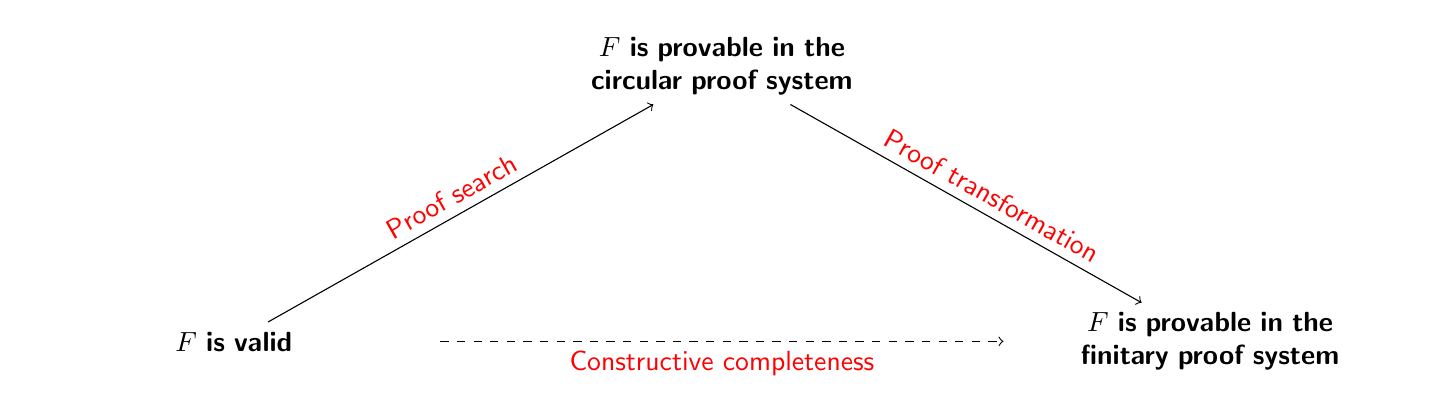
\begin{tikzpicture}
    \node [text width=5cm,text centered] (1) at (0,3.5) [] {\textbf{$F$ is provable in the circular proof system}};
    \node[text width=5cm,text centered] (0) at (-6.2,0) [] {\textbf{$F$ is valid}};
   \node[text width=5cm,text centered] (2) at (6.2,0) [] {\textbf{$F$ is provable in the finitary proof system}};
    \draw [->] (0) to node [above, sloped] {\textcolor{red}{Proof search}} (1);
    \draw[->]  (1) to node [above, sloped] {\textcolor{red}{$\quad$ Proof transformation}} (2);
 \draw [->,dashed] (0) to node [below] {\textcolor{red}{Constructive completeness}} (2);
\end{tikzpicture}
\end{flushleft}
\caption{Schema of constructive proof of completeness  \label{ConstructiveCompleteness}}
\end{figure*}

The interest of this proof schema is that it allows proofs of completeness which are ``constructive'', meaning that they do not only establish that every valid formula is provable, but they also give a concrete proof of this formula. Indeed, circular proof systems are more adapted to proof search, thus it is generally easier to  \textbf{construct}
a circular proof for each valid formula. It is then enough to transform the obtained proof into a proof of the target proof system using the algorithms that we hope to obtain by solving Problem 4.


\begin{center}
\begin{bclogo}[logo= ,arrondi = 0.1, couleur = green!10,  epBarre = 0]{}
  \vspace{-10pt}
  \textbf{Problem 5.}

Show completeness in a constructive way using circular proofs.
  %\vspace{5pt}
\end{bclogo}
\end{center}

I succeeded in instantiating this proof schema in two  frameworks: the first is  linear time $\mu$-calculus, showing in a constructive and direct way Kaivola's result~\cite{}; the second in Kleene algebras, showing in a simple way Kozen and Silva's result~\cite{}. The hope is to show, using this technique, completeness for logics for which this result is still open (extensions of Kleene algebras for instance, such as Kleene allegories and nominal Kleene
algebras).


\paragraph{C3: Comparing with respect to computational content}

If we wear Curry-Howard glasses, a proof denotes a program and a proof system denotes a class
of programs. Another question that arises naturally is to find wich class of programs circular and finitary proof sytems correspond to, and whether they denote the same set of programs.

\begin{center}
\begin{bclogo}[logo= ,arrondi = 0.1, couleur = green!10,  epBarre = 0]{}
  \vspace{-10pt}
  \textbf{Problem 6.}

Do circular and finitary proof systems have the same computational content?
\end{bclogo}
\end{center}

Comparing the provability power and the computational power of  circular and finitary proof systems are not disconnected problematics. Indeed, the algorithms of proof transformation used to establish the equivalence between the principles of infinite descente and (co)inductive reasonning can be used as tools to compare circular and finitary proof systems from the computational point of view: we could, for instance, show that those algorithms preserve the computational content of proofs.


\smallskip

Answering Problem 6 necessarily goes through the study of the cut-elimination property.
Showing this property in a circular/infinitary setting will probably require new proof techniques. Indeed, proofs of cut-elimination usually proceeds by induction on the proof, or at least rely on the fact that they are finite objects.
My PhD work opens some ways in this direction, but now the question is: can we generalize these ideas to other frameworks? To other kind of proof systems such as natural deduction?


\bigskip

This first axis being in the continuity of my PhD work, I see it more as a short to medium term goal.

\paragraph{2.5\ Academic impact.}

\jbcomment{I will write the first draft of this part}


%% Again, aim for about one column of references.
\newpage
{\footnotesize
\begin{spacing}{0.9}
\bibliographystyle{plain}
\bibliography{biblio}
\end{spacing}}


\end{document}


